%% Post-Quantum Edge Communication
%% Author: Devesh Kumar, Indian Institute of Technology Ropar
%% devesh.kumar.csm2024@iitrpr.ac.in
%% Build: pdflatex main && bibtex main && pdflatex main && pdflatex main
\documentclass[conference]{IEEEtran}
\IEEEoverridecommandlockouts

\usepackage{cite}
\usepackage{amsmath,amssymb,amsfonts}
\usepackage{graphicx}
\usepackage{booktabs}
\usepackage{xcolor}
\usepackage{url}
\usepackage[hidelinks]{hyperref}
\usepackage{algorithm}
\usepackage{algorithmic}
\usepackage{microtype}

\graphicspath{{figures/}}

\begin{document}

\title{Neural Synchronization Meets 5G Split Bearers: ML-KEM-Anchored Security for Resource-Constrained Edge Devices}

% \author{%
% \IEEEauthorblockN{Devesh Kumar}
% \IEEEauthorblockA{Department of Computer Science and Engineering\\
% Indian Institute of Technology Ropar\\
% Rupnagar, Punjab 140001, India\\
% devesh.kumar.csm2024@iitrpr.ac.in}}

% \author{
% \IEEEauthorblockN{
% Devesh Kumar,
% Dr. S. K. Pal
% }

% \IEEEauthorblockA{
% Defence Research and Development Organisation (DRDO), Delhi, India\\
% Email: devesh.kumar.hqr@gov.in, saibal.pal@gov.in
% }
% }
\author{
\IEEEauthorblockN{
Anonymous Author1,
Anonymous Author2
}

\IEEEauthorblockA{
Prepared for double-blind review\\
Email: Prepared for double-blind review
}
}

\maketitle

\begin{abstract}
Edge nodes on 5G links face three simultaneous demands: agree on a
key with the core, carry payload across links they do not fully control, and remain
observable enough that someone can actually catch an attack---all while the industry
is mid-migration to post-quantum cryptography. We describe a framework that keeps
these concerns separate but coordinated. Key establishment is anchored in ML-KEM
(FIPS~203), which carries the post-quantum guarantee; a Tree-Parity-Machine (TPM)
neural-synchronization step is folded in only as defence-in-depth via a
concatenation KDF, never as the primary basis of confidentiality. Payloads are
distributed across multiple 5G carriers with a tunable $(T,N)$ Shamir threshold
scheme, letting an operator dial the confidentiality--availability trade-off rather
than accept the fixed $(2,2)$ XOR behaviour. A hybrid weighted-$k$NN plus
feed-forward detector then watches both cryptographic and transport telemetry and
flags active attacks versus network faults. We are straightforward about what the
results show: TPM loses a head-to-head benchmark against ML-KEM on both latency and
provability, and its only surviving advantage is wire footprint (about 73 bytes vs.\
ML-KEM's 2\,272). On the detection side, cross-modal fusion is what moves the needle
---any reasonable classifier climbs from macro-F1 near $0.40$--$0.49$ on one
telemetry modality to roughly $0.90$ on both---and no classifier is statistically
better than any other on the same features. Code, a grounded data generator, a
5G-NIDD adapter, and a Jetson Orin Nano deployment path accompany the paper.
\end{abstract}

\begin{IEEEkeywords}
post-quantum cryptography, ML-KEM, neural cryptography, tunable secret sharing,
5G edge security, anomaly detection, cross-modal feature fusion.
\end{IEEEkeywords}

% ============================================================
\section{Introduction}
% ============================================================
A 5G edge node lives with three problems at once. It must agree on a key with the
core, it must carry traffic over links it does not fully control, and somebody needs
to be able to tell, after the fact, whether anything went wrong. None of this is new.
What has changed is the urgency: harvest-now-decrypt-later attacks and the approach
of cryptographically relevant quantum computers~\cite{shor1997polynomial} mean key
agreement now has to be post-quantum, and standards bodies have responded quickly.
NIST finalized ML-KEM, ML-DSA, and SLH-DSA in 2024~\cite{fips203,fips204,fips205},
and NSA's CNSA~2.0 timeline is already pushing networking equipment toward exclusive
post-quantum use~\cite{cnsa2}.

Against that backdrop there is a steady stream of work proposing Tree-Parity-Machine
(TPM) neural synchronization~\cite{kanter2002secure,rosenzvi2002mutual} as a
lightweight key-agreement candidate for constrained links, and a worrying fraction of
it claims or implies quantum resistance---recent smart-grid and IoT proposals
explicitly market TPM as a post-quantum alternative~\cite{stypinski2023smartgrid}.
That claim does not hold. TPM has no reduction to a hard problem, and geometric,
genetic, and majority attacks that break it have been in the literature for more than
twenty years~\cite{klimov2002analysis,ruttor2006genetic,shacham2004cooperating}. The
honest response is not to abandon the idea but to place it where it actually earns
its keep.

This paper builds and measures a framework that does exactly that. Post-quantum
security comes entirely from ML-KEM. The TPM step is kept only as defence-in-depth
---extra entropy with an unusually small public-channel footprint---combined with the
ML-KEM secret via a NIST SP~800-56C concatenation KDF~\cite{sp80056c} so the
session key is no weaker than its strongest component~\cite{stebila2023hybrid}. On
that key we place a transport layer that splits payloads across 5G carriers with a
tunable $(T,N)$ threshold scheme, and a machine-learning detector that fuses both
telemetry streams for runtime observability.

\noindent\textbf{Contributions.}
\begin{itemize}
\item A hybrid key-establishment design that anchors post-quantum security in ML-KEM
and demotes TPM to auxiliary entropy, backed by an honest head-to-head benchmark
showing ML-KEM is faster \emph{and} proven (Table~\ref{tab:pqc}).
\item A privacy-preserving, rate-limited early-termination protocol for the TPM step
that cuts verification traffic roughly five-fold at no cost to key agreement
(Table~\ref{tab:earlyterm}).
\item Tunable $(T,N)$ secret sharing over $\mathrm{GF}(2^8)$ that generalizes the
fixed $(2,2)$ split and exposes the confidentiality--availability frontier as an
operator-configurable knob (Fig.~\ref{fig:tn}).
\item Clear evidence that cross-modal \emph{fusion}---not classifier
choice---explains detector performance: every baseline we tested landed within noise,
and the gap is not statistically significant (Table~\ref{tab:baselines}).
\item A fully reproducible artifact: grounded synthetic data generator, 5G-NIDD
adapter, all experiments and figures, and a Jetson Orin Nano deployment path.
\end{itemize}

% ============================================================
\section{Related Work}
% ============================================================

\textbf{Post-quantum key establishment.}
ML-KEM~\cite{fips203} is an IND-CCA2 KEM whose security reduces to Module-LWE.
Migration guidance favours hybrid schemes that concatenate a classical and a
post-quantum secret in a KDF, secure if either component is~\cite{sp80056c,
stebila2023hybrid}; IKEv2 encodes the same idea~\cite{rfc9370}. Our hybrid pairs
ML-KEM with a neural-synchronization secret, which lets us measure what, concretely,
the neural component adds---and, more importantly, what it does not.

\textbf{Neural cryptography.}
TPM synchronization was proposed in~\cite{kanter2002secure} and studied
in~\cite{rosenzvi2002mutual}. Klimov, Mityagin, and Shamir broke it three
ways~\cite{klimov2002analysis}; genetic and majority attacks
followed~\cite{ruttor2006genetic,shacham2004cooperating,ruttor2007neural}, and even
the later permutation-parity extensions have been
compromised~\cite{seoane2012successful}. More elaborate ``real-life
systems''~\cite{jeong2021generalized} still carry no security reduction. We treat
this literature as settled: TPM is not a stand-alone secure primitive, and framing it
as post-quantum~\cite{stypinski2023smartgrid} is an overreach.

\textbf{Secret sharing and path diversity.}
Shamir's scheme~\cite{shamir1979share} is the foundation. Spreading shares over
disjoint paths for confidentiality was explored in ad-hoc
routing~\cite{lou2004spread} and multipath TCP~\cite{jadin2017securing}; 5G's PDCP
split bearer~\cite{tgpp38323} provides the substrate. Most prior work fixes the
split; we parametrize it and quantify the trade-off.

\textbf{ML-based anomaly detection.}
The field has shifted from classical learners~\cite{cover1967nearest,hastie2009elements}
toward deep models~\cite{lecun2015deep} on datasets such as UNSW-NB15~\cite{moustafa2015unsw},
CICIDS2017~\cite{sharafaldin2018toward}, and TON\_IoT~\cite{alsaedi2020toniot}. For
5G specifically, 5G-NIDD~\cite{samarakoon2022nidd} provides labelled attack traffic
from a real test network. The 5G edge also introduces its own attack surface at the
MEC layer~\cite{ranaweera2021mec,tgpp33501}. Our detector is deliberately simple;
the methodological point we want to make is about fusion and significance, not about
a new architecture.

% ============================================================
\section{System and Threat Model}
% ============================================================

An edge node and a core gateway run ML-KEM to establish a 32-byte shared secret,
optionally run the TPM step in parallel, and derive the session key from both via the
hybrid KDF (Section~\ref{sec:hybrid}). Payloads are split into $N$ shares by a
$(T,N)$ threshold scheme and sent over $N$ 5G legs; any $T$ arriving shares
reconstruct. A detector at the edge node consumes telemetry from both layers and
classifies each session.

We assume a Dolev--Yao adversary~\cite{dolev1983security} that sees all public
messages and may inject or probe. Against ML-KEM it gains nothing without solving
Module-LWE. Against the TPM step it may run its own machines including a majority
ensemble. One limitation stated upfront: a purely passive eavesdropper leaves no
host-side artifact and is therefore invisible to our telemetry detector. We model
attack classes as active (injection, probing, traffic shaping), which perturb
observable signals such as round count, key match probability, and flow statistics.
Detection complements cryptography here; it is not a substitute for it.

% ============================================================
\section{Methodology}
% ============================================================

\subsection{Hybrid ML-KEM + TPM Key Establishment}
\label{sec:hybrid}

The initiator generates $(ek, dk)$, sends $ek$ to the responder, who encapsulates
and returns ciphertext $ct$ along with $ss_{\mathrm{pq}}$; the initiator
decapsulates to recover the same $ss_{\mathrm{pq}}$. In parallel, if the TPM branch
is enabled, both parties synchronize tree parity machines ($K$ hidden units, $N$
inputs each, weights in $[-L,L]$) and derive a second secret $ss_{\mathrm{tpm}}$
from the agreed weight matrices. The session key is

\begin{equation}
k = \mathrm{HKDF}\!\left(\,\mathrm{len}(ss_{\mathrm{pq}})\|ss_{\mathrm{pq}}\|
\mathrm{len}(ss_{\mathrm{tpm}})\|ss_{\mathrm{tpm}},\;\ell\right),
\label{eq:hkdf}
\end{equation}

\noindent where $\ell$ is a domain-separation label and ML-KEM is placed first so
that a FIPS-approved secret seeds the extraction step. The key property follows
directly from the HKDF construction: $k$ is secure as long as \emph{either} input
is, so the hybrid cannot be weaker than ML-KEM alone~\cite{sp80056c}. We treat
$ss_{\mathrm{tpm}}$ strictly as auxiliary; it must never be the sole basis for
confidentiality. Algorithm~\ref{alg:hybrid} gives the full protocol.

\begin{algorithm}[t]
\small
\caption{Hybrid Key Establishment}
\label{alg:hybrid}
\begin{algorithmic}[1]
\REQUIRE ML-KEM level $\ell$; TPM config $(K,N,L)$; flag \texttt{use\_tpm}
\ENSURE 32-byte session key $k$
\STATE $ek,\,dk \leftarrow \texttt{ML-KEM}_\ell.\texttt{KeyGen}()$
    \COMMENT{initiator}
\STATE send $ek$ to responder
\STATE $ss_{\mathrm{pq}},\,ct \leftarrow \texttt{ML-KEM}_\ell.\texttt{Encaps}(ek)$
    \COMMENT{responder encapsulates}
\STATE send $ct$ to initiator
\STATE $ss_{\mathrm{pq}} \leftarrow \texttt{ML-KEM}_\ell.\texttt{Decaps}(dk,ct)$
    \COMMENT{initiator recovers secret}
\IF{\texttt{use\_tpm}}
  \REPEAT
    \STATE exchange $x \in \{{\pm}1\}^{K\times N}$; both parties run forward + update
    \STATE track windowed agreement rate and consecutive-streak count
  \UNTIL{confidence $\geq\tau$ AND streak $\geq\sigma$ AND cooldown elapsed}
  \STATE verify: $\texttt{HMAC}(\texttt{SHA256}(W_A),n)\;\stackrel{?}{=}\;\texttt{HMAC}(\texttt{SHA256}(W_B),n)$
        \COMMENT{leaks ${\leq}1$ bit}
  \STATE $ss_{\mathrm{tpm}} \leftarrow \texttt{HKDF}(W.\text{bytes},\;\text{``pqedge-tpm''})$
\ELSE
  \STATE $ss_{\mathrm{tpm}} \leftarrow \varepsilon$
\ENDIF
\RETURN $k$ via Eq.~(\ref{eq:hkdf})
\end{algorithmic}
\end{algorithm}

\textbf{Privacy-preserving early termination (steps 7--11).}
Both parties track a confidence signal derived only from public outputs: the windowed
fraction of agreeing rounds and the current consecutive-agreement streak. Once both
cross their thresholds and a cooldown has elapsed, they exchange
$\texttt{HMAC}(\texttt{SHA256}(\text{weights}),\,\text{nonce})$ over a fresh
public nonce. Equal tags imply equal weight matrices with overwhelming probability
while leaking at most one equality bit. The cooldown prevents a prolonged
high-confidence plateau before true synchronization from repeatedly triggering
the check.

\subsection{Tunable $(T,N)$ Multi-Carrier Bifurcation}

Rather than the fixed $(2,2)$ XOR split, we apply Shamir's scheme over
$\mathrm{GF}(2^8)$~\cite{shamir1979share}: a payload becomes $N$ shares such that
any $T$ reconstruct it and any $T-1$ reveal nothing (information-theoretically). Each
share rides one 5G leg modelled as a PDCP split bearer~\cite{tgpp38323}. With
independent per-PDU loss $p$ and $n$ PDUs per share, each leg succeeds with
probability $q=(1-p)^{n}$, and reconstruction succeeds when at least $T$ legs arrive:

\begin{equation}
A(T,N)=\sum_{k=T}^{N}\!\binom{N}{k}q^{k}(1-q)^{N-k}.
\label{eq:avail}
\end{equation}

Setting $T{=}1,N{=}1$ gives a single carrier; $T{=}2,N{=}2$ is the maximally
confidential XOR split; $T{=}1,N{=}2$ is duplication. The confidentiality threshold
is $T$ (an adversary needs at least $T$ carriers to learn anything) and the
availability margin is $N-T$ (that many legs can fail without losing the payload).

\subsection{Cross-Modal Anomaly Detector}

Each session is summarised by ten features: four cryptographic (TPM convergence,
sync rate, key match probability, normalized round count) and six transport
(end-to-end latency, per-PDU loss, throughput, jitter, share reconstruction
failures, flow volume). A weighted $k$NN ($k{=}15$, inverse-distance weights) and a
small feed-forward network (two hidden layers of 64--32 units, ReLU, dropout 0.1)
are fused by soft voting:
$p = \alpha\,p_{\text{FNN}}+(1-\alpha)\,p_{k\text{NN}}$.
The output is one of six classes: \textit{Normal}, \textit{Geometric attack},
\textit{Majority attack}, \textit{Injection}, \textit{Carrier fault}, and
\textit{Traffic manipulation}. The design is kept lightweight so it can run
on an edge node; the architectural choices themselves are not the claimed contribution.

% ============================================================
\section{Experimental Setup}
% ============================================================

All runs are on CPU, reproducibly seeded. ML-KEM uses a pure-Python FIPS~203
reference implementation (kyber-py v1.2); because Python object overhead dominates,
the absolute timings are not representative of hardware---we read them only
relatively and quote standardized, implementation-independent byte sizes for wire
cost. Optimized on-device numbers need hardware-specific
assembly~\cite{kannwischer2019pqm4}. The detector trains on a grounded synthetic
dataset in which cryptographic features are bootstrapped from real TPM sessions and
transport features from real PDCP transmissions, with documented per-class magnitude
shifts, additive Gaussian noise, and 3\% label noise. We also provide a 5G-NIDD
adapter~\cite{samarakoon2022nidd}; because that dataset carries only transport
telemetry, the cryptographic features must be augmented synthetically to run the
fusion path, and we flag that explicitly. Unless stated otherwise: $K{=}3$, $N{=}100$,
$L{=}4$; security rates average over at least 25 decorrelated sessions; detection
results use a stratified 75/25 split repeated over three seeds.

\begin{table}[t]
\centering
\caption{Key establishment: standardized ML-KEM vs the TPM neural key-agreement candidate vs the hybrid. ML-KEM timings are a \emph{pure-Python reference} (relative only); byte sizes are standardized (FIPS~203). TPM's sole advantage is wire footprint; it carries no security proof.}
\label{tab:pqc}
\begin{tabular}{lcccc}
\toprule
Scheme & Estab. (ms) & Wire (B) & Secret (B) & Proof \\
\midrule
ML-KEM-512 & 9.918 & 1568 & 32 & yes \\
ML-KEM-768 & 14.749 & 2272 & 32 & yes \\
ML-KEM-1024 & 22.173 & 3136 & 32 & yes \\
TPM(K=3,N=80,L=4) & 61.769 & 73 & 32 & no \\
\midrule
Hybrid (768+TPM) & 72.701 & 2345 & 32 & yes \\
\bottomrule
\end{tabular}
\end{table}


\begin{table}[t]
\centering
\caption{Cumulative ablation of the framework components. Crypto columns use $K{=}3,N{=}100$; eavesdropper success is the operational (majority-vote) key-recovery rate; availability is the (2,2) reconstruction probability at per-PDU loss $p{=}0.05$.}
\label{tab:configs}
\resizebox{\columnwidth}{!}{%
\begin{tabular}{lccccc}
\toprule
Config & Verif. & Att.$_{geo}$ & Att.$_{maj}$ & Avail. & F1 \\
\midrule
TPM baseline & 10.200 & 0.520 & 0.000 & -- & -- \\
+ Early term. & 1.840 & 0.360 & 0.000 & -- & -- \\
+ Bifurcation & 1.840 & 0.360 & 0.000 & 0.440 & -- \\
+ Anomaly det. & 1.840 & 0.360 & 0.000 & -- & 0.901 \\
Complete & 1.840 & 0.360 & 0.000 & 0.440 & 0.901 \\
\bottomrule
\end{tabular}}
\end{table}

\begin{table}[t]
\centering
\caption{Effect of privacy-preserving early termination versus fixed-interval verification, against the geometric eavesdropper ($K{=}3,N{=}100$). Rate-limited verification bounds the message count.}
\label{tab:earlyterm}
\begin{tabular}{lccc}
\toprule
Policy & Rounds & Verif. & Att.$_{geo}$ \\
\midrule
hash-only & 467.5 & 9.350 & 0.450 \\
early ($\tau{=}0.95$) & 510.5 & 2.600 & 0.400 \\
early ($\tau{=}0.98$) & 513.9 & 1.800 & 0.400 \\
early ($\tau{=}0.99$) & 513.9 & 1.800 & 0.400 \\
\bottomrule
\end{tabular}
\end{table}


% ============================================================
\section{Results and Discussion}
% ============================================================

\subsection{Key Establishment: What TPM Actually Buys}

Table~\ref{tab:pqc} is the result that reframes the whole design. Even with the
overhead of pure-Python dispatch, ML-KEM establishes a shared key faster than our
TPM step does---and ML-KEM comes with a security argument that TPM simply does not
have. The neural scheme wins on exactly one axis: bytes exchanged over the public
channel, where roughly one bit per synchronization round produces tens of bytes
against ML-KEM's one-to-three kilobytes. That is a real, if narrow, advantage on
extremely bandwidth-constrained links, and it is the only honest reason to keep the
TPM step at all---strictly as auxiliary entropy inside the hybrid, never as a
replacement for ML-KEM. The hybrid costs roughly the sum of its parts (72.7\,ms at
N\,=\,80), with an otherwise negligible KDF step, and inherits ML-KEM's guarantee
unconditionally.


\subsection{Early Termination and Security}

Table~\ref{tab:configs} presents the five cumulative configurations C1--C5.
Switching from fixed-interval hash verification (C1) to confidence-gated stopping
(C2) cuts the mean verification-message count from about ten to under two per
session while synchronization rounds change by less than 2\% and key agreement
stays at 100\%. Table~\ref{tab:earlyterm} shows how the count and the geometric
attacker's success change as we tighten the confidence threshold: at $\tau{=}0.95$
the count drops to 2.6; tightening to $\tau{=}0.98$ reaches 1.8 with no further
change to attacker success, and the rate-limiting kicks in to keep it there.
Without that cooldown, a prolonged high-confidence plateau before true weight
equality would keep triggering the check and the savings would evaporate.

The geometric eavesdropper still succeeds with non-negligible probability (${\sim}0.40$)
at $K{=}3$---we do not hide that. The majority ensemble reaches high overlap but
stays below the key-recovery threshold, which is precisely why the design never
leans on TPM alone. Fig.~\ref{fig:sync} illustrates a typical session: the two
parties converge while the attacker's overlap climbs but cannot match.

\begin{figure}[t]
\centering
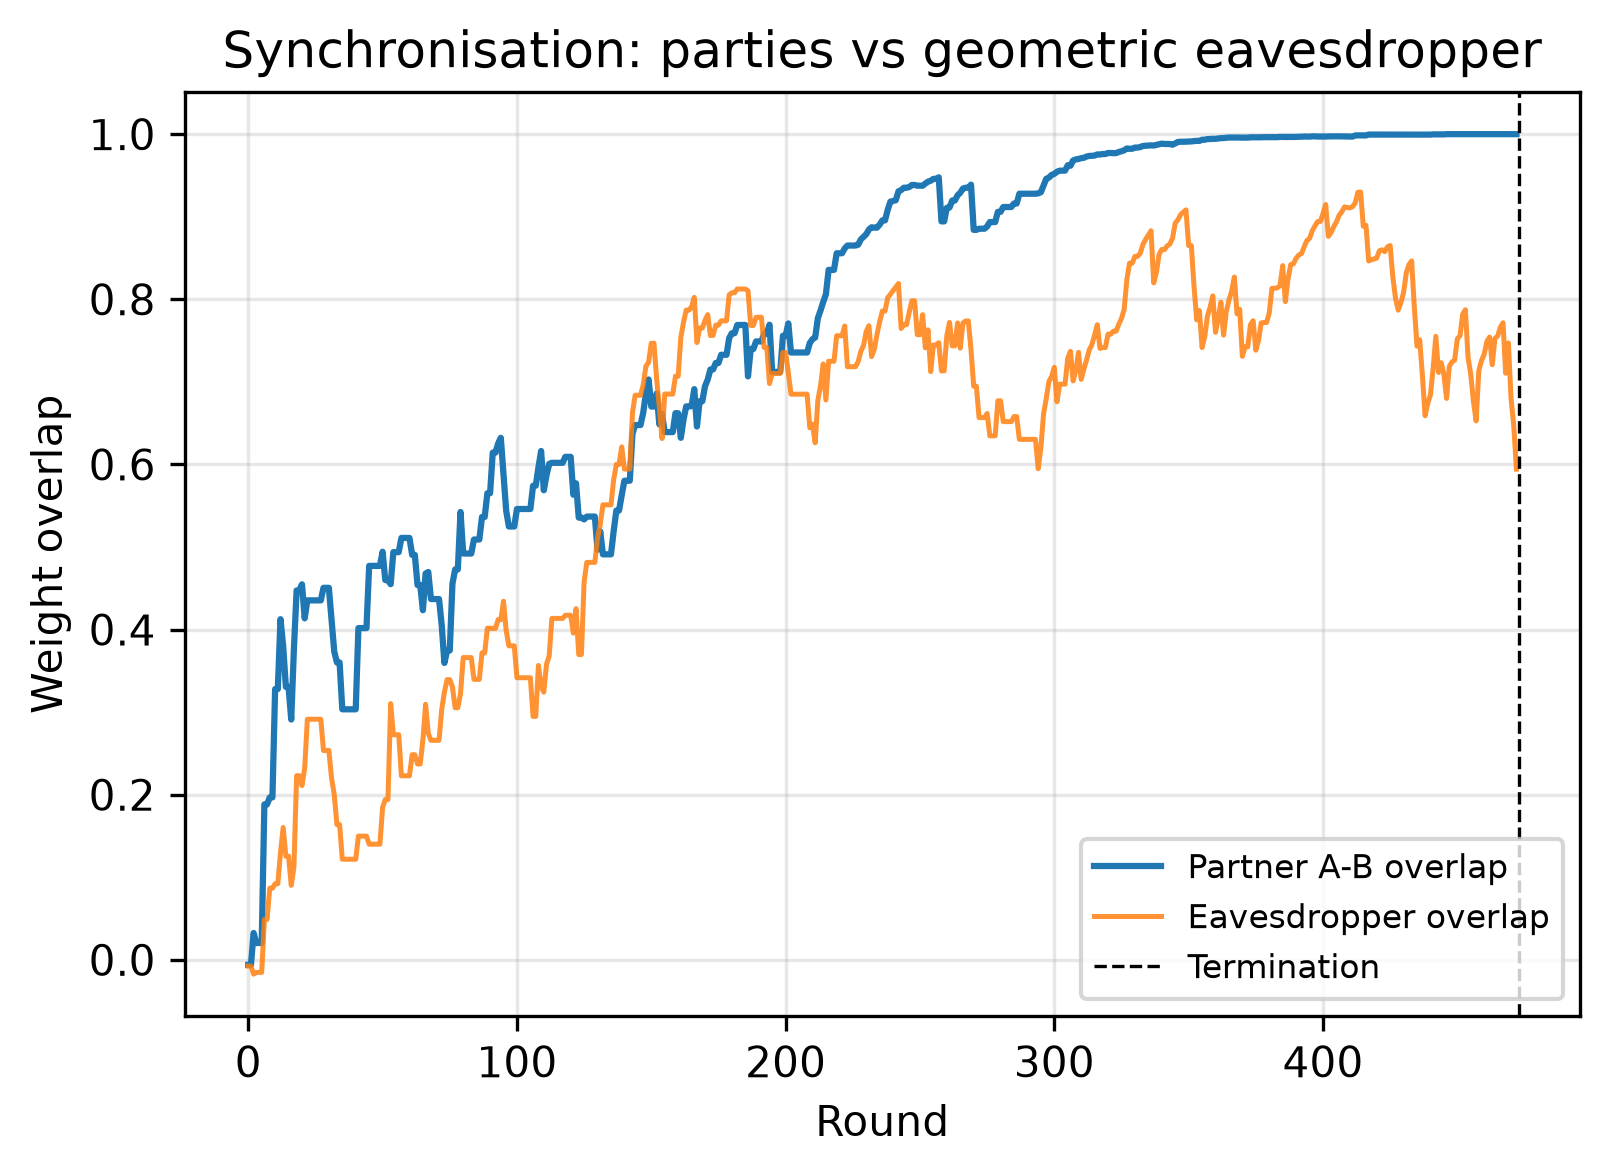
\includegraphics[width=0.49\columnwidth]{sync_trace.png}\hfill
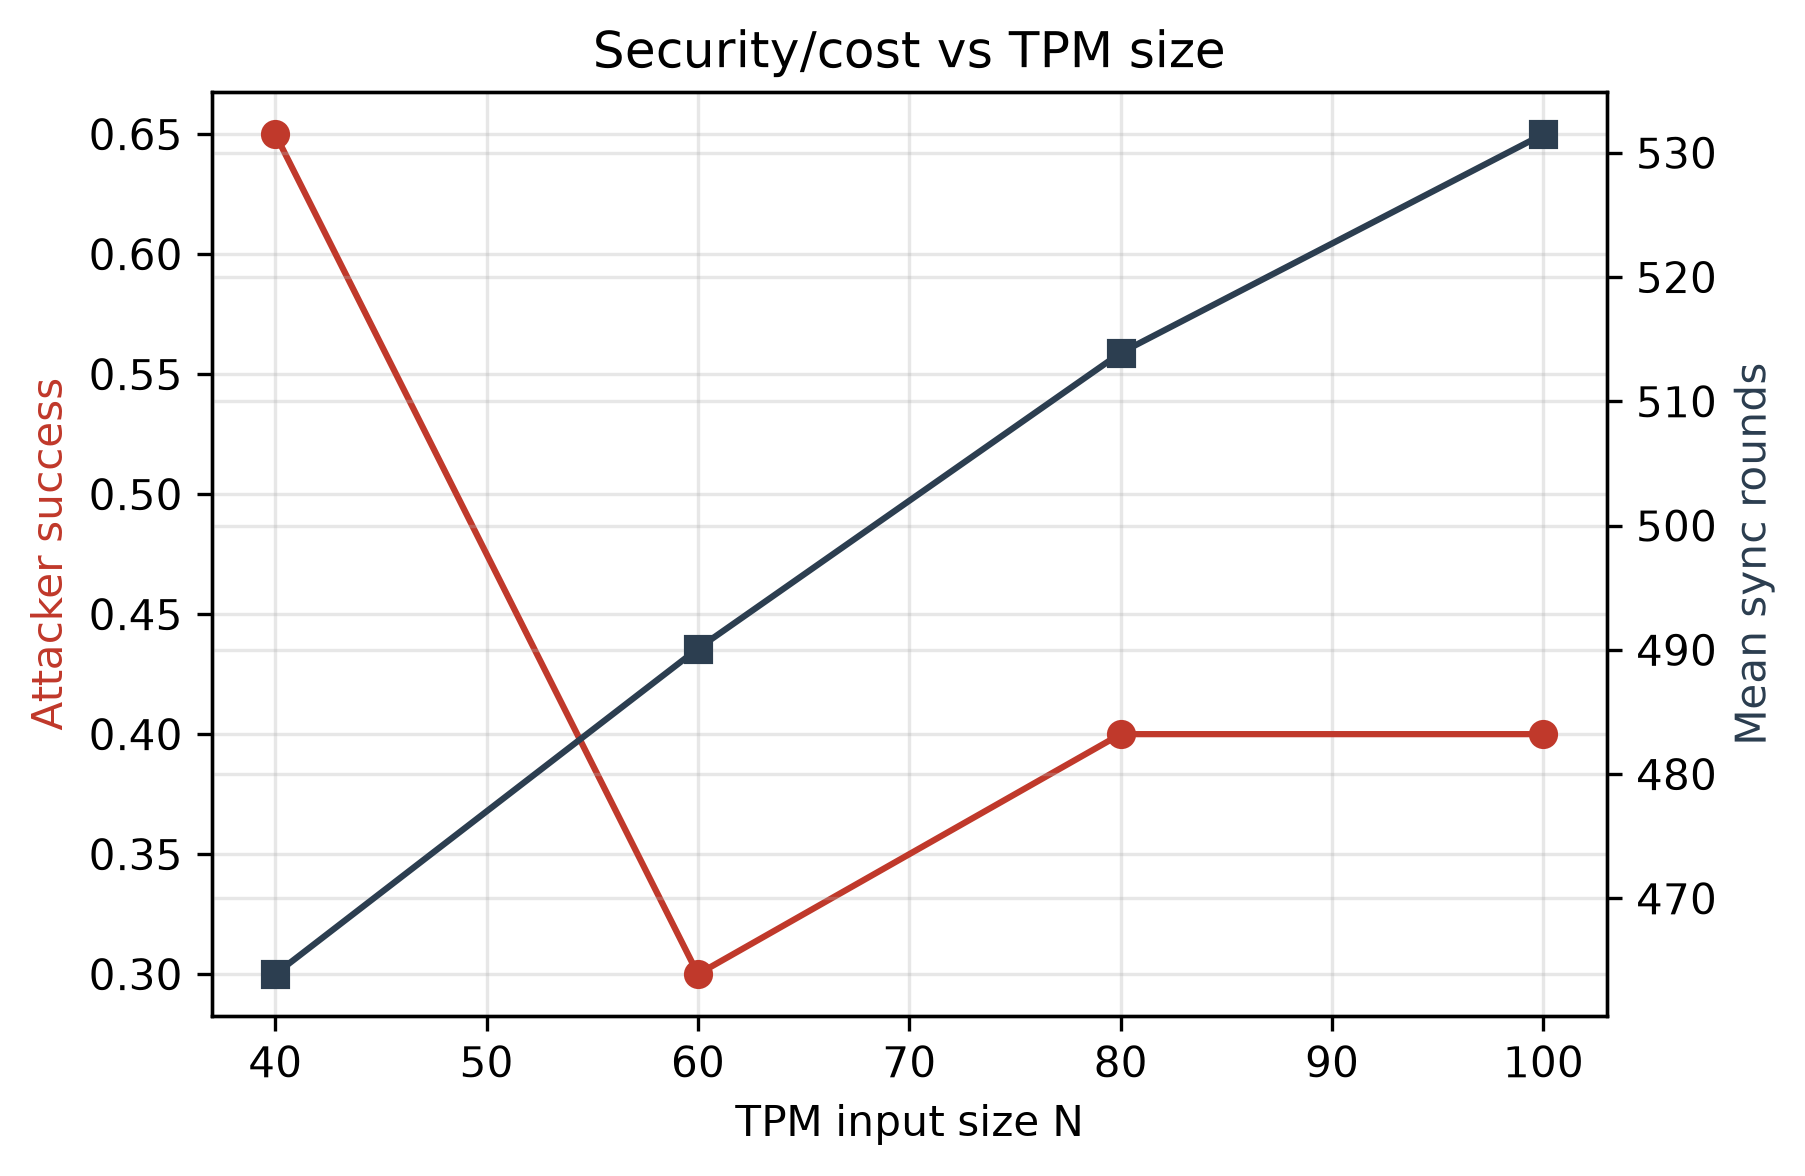
\includegraphics[width=0.49\columnwidth]{sweep_tpm_N.png}
\caption{Left: a single synchronization session; partner overlap (A--B) converges
to 1.0 while the geometric eavesdropper's overlap rises but stays sub-threshold.
Right: geometric-attacker success and mean synchronization rounds vs.\ TPM input
size $N$ at $K{=}3$. Larger $N$ helps, noisily, but is not a substitute for the
ML-KEM anchor.}
\label{fig:sync}
\end{figure}

\subsection{Tunable $(T,N)$ Bifurcation}

Table~\ref{tab:reliability} fixes the three canonical strategies at $p{=}0.05$, 8
PDUs per share. The $(2,2)$ split almost halves availability relative to a single
carrier (0.44 vs.\ 0.66) while duplication more than recovers it (0.89). The
$(T,N)$ abstraction makes this a sliding scale. Fig.~\ref{fig:tn} sweeps $T$ from 1
to 5 at $N{=}5$: availability drops from 0.996 at $(1,5)$ to 0.129 at the
maximally confidential $(5,5)$, passing through 0.953, 0.785, and 0.455. A
deployment with three modems could pick $(2,3)$ for meaningful redundancy and still
require an adversary to compromise two carriers before learning anything---a much
better operating point than the fixed $(2,2)$ scheme forces.

\begin{table}[t]
\centering
\caption{Transport reliability at per-PDU loss $p{=}0.05$, 8 PDUs per share. (2,2) bifurcation maximises confidentiality but lowers availability; duplication recovers availability at the cost of confidentiality.}
\label{tab:reliability}
\begin{tabular}{lcc}
\toprule
Scheme & Analytic avail. & MC avail. \\
\midrule
Single carrier & 0.663 & -- \\
(2,2) split bearer & 0.440 & 0.450 \\
Duplicated (2 of 2) & 0.887 & -- \\
\bottomrule
\end{tabular}
\end{table}


\begin{figure}[t]
\centering
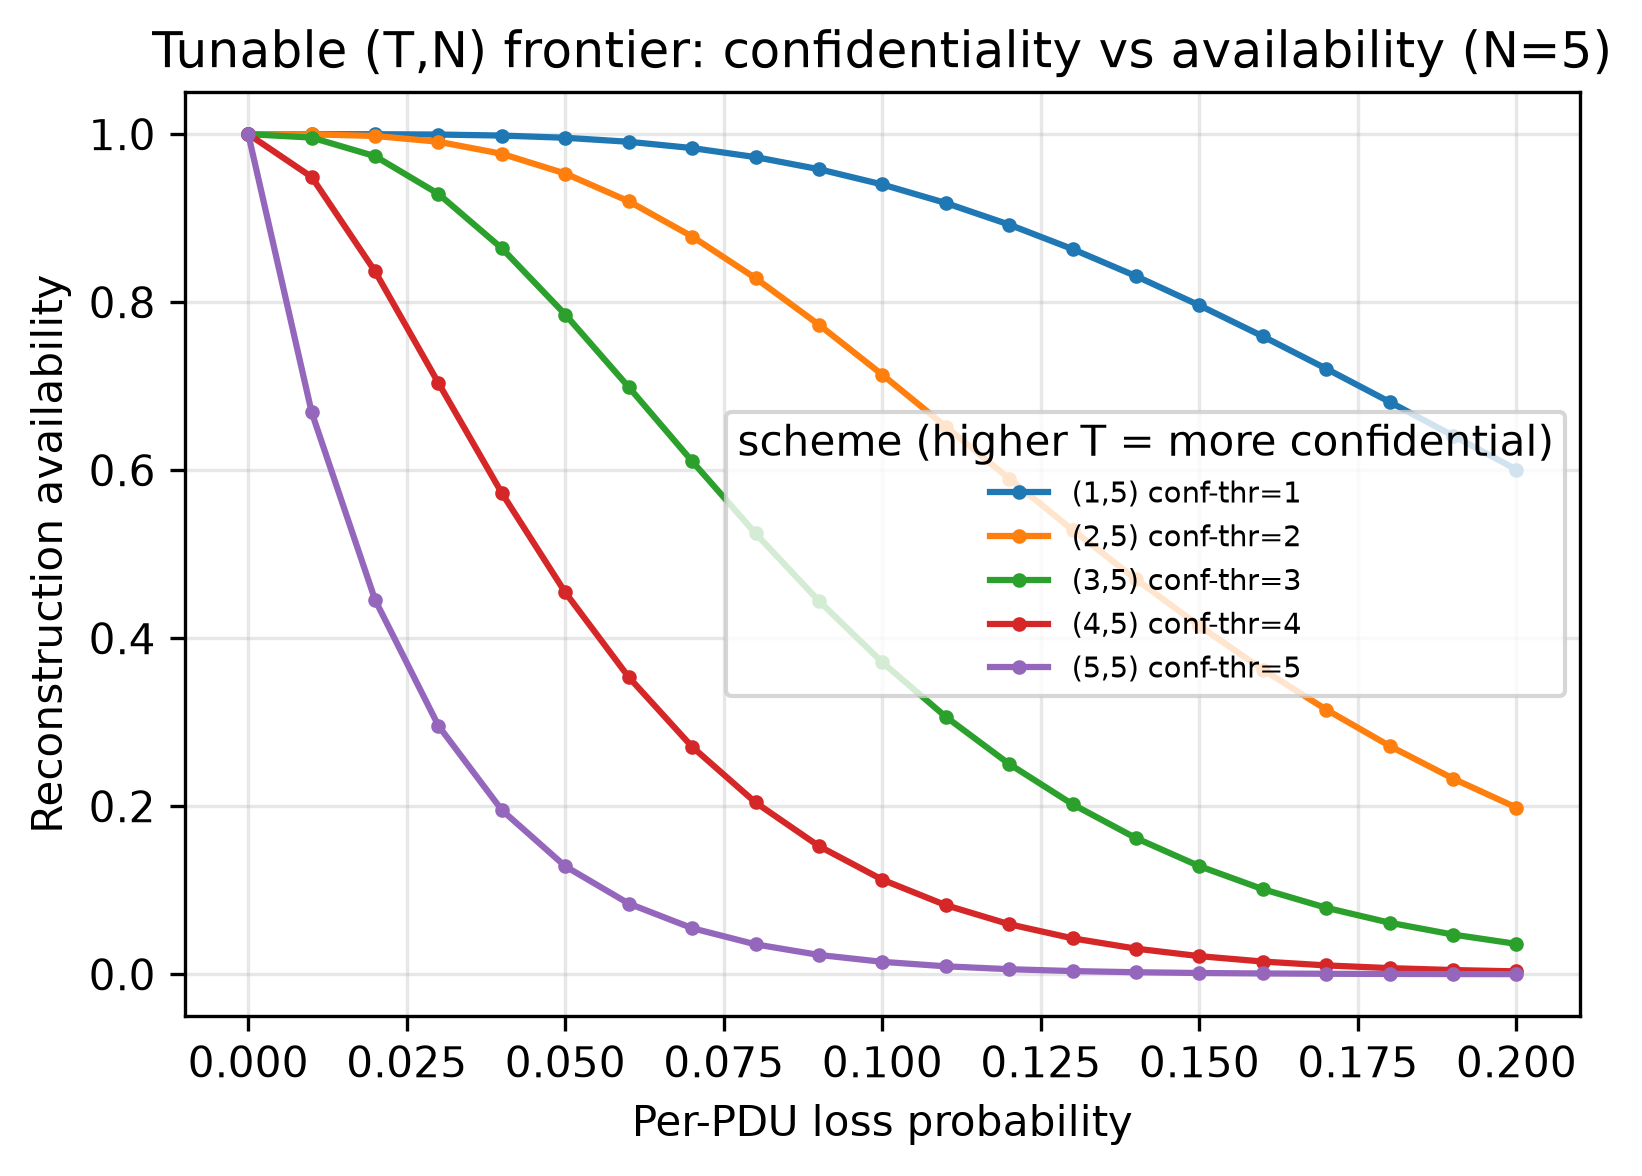
\includegraphics[width=0.90\columnwidth]{threshold_frontier.png}
\caption{$(T,N)$ confidentiality--availability frontier at $N{=}5$, $p{=}0.05$,
8 PDUs per share. Higher $T$ raises the number of carriers an adversary must capture
to learn the payload and simultaneously tightens the tolerance to link loss.}
\label{fig:tn}
\end{figure}

\subsection{Detection: Fusion Beats Architecture}

The central finding is in Table~\ref{tab:detector} and Fig.~\ref{fig:det}.
Restricting to cryptographic features alone gives macro-F1 of 0.41; transport
features alone give 0.50; combining both reaches 0.91. Neither view is sufficient
on its own because distinguishing a cryptographic attack from an ordinary carrier
fault genuinely needs both kinds of evidence---they look very similar in any single
modality.

\begin{table}[t]
\centering
\caption{Detector ablations on the held-out test split. Left: architecture. Right: feature-group restriction (non-selected features zeroed). Neither cryptographic nor transport telemetry alone suffices; their fusion drives performance.}
\label{tab:detector}
\begin{tabular}{lcc@{\hskip 1.5em}lcc}
\toprule
Model & F1 & AUC & Features & F1 & AUC \\
\midrule
WKNN & 0.896 & 0.972 & Crypto & 0.415 & 0.826 \\
FNN & 0.913 & 0.977 & Transport & 0.500 & 0.862 \\
Hybrid & 0.906 & 0.977 & All & 0.909 & 0.977 \\
\bottomrule
\end{tabular}
\end{table}


\begin{figure}[t]
\centering
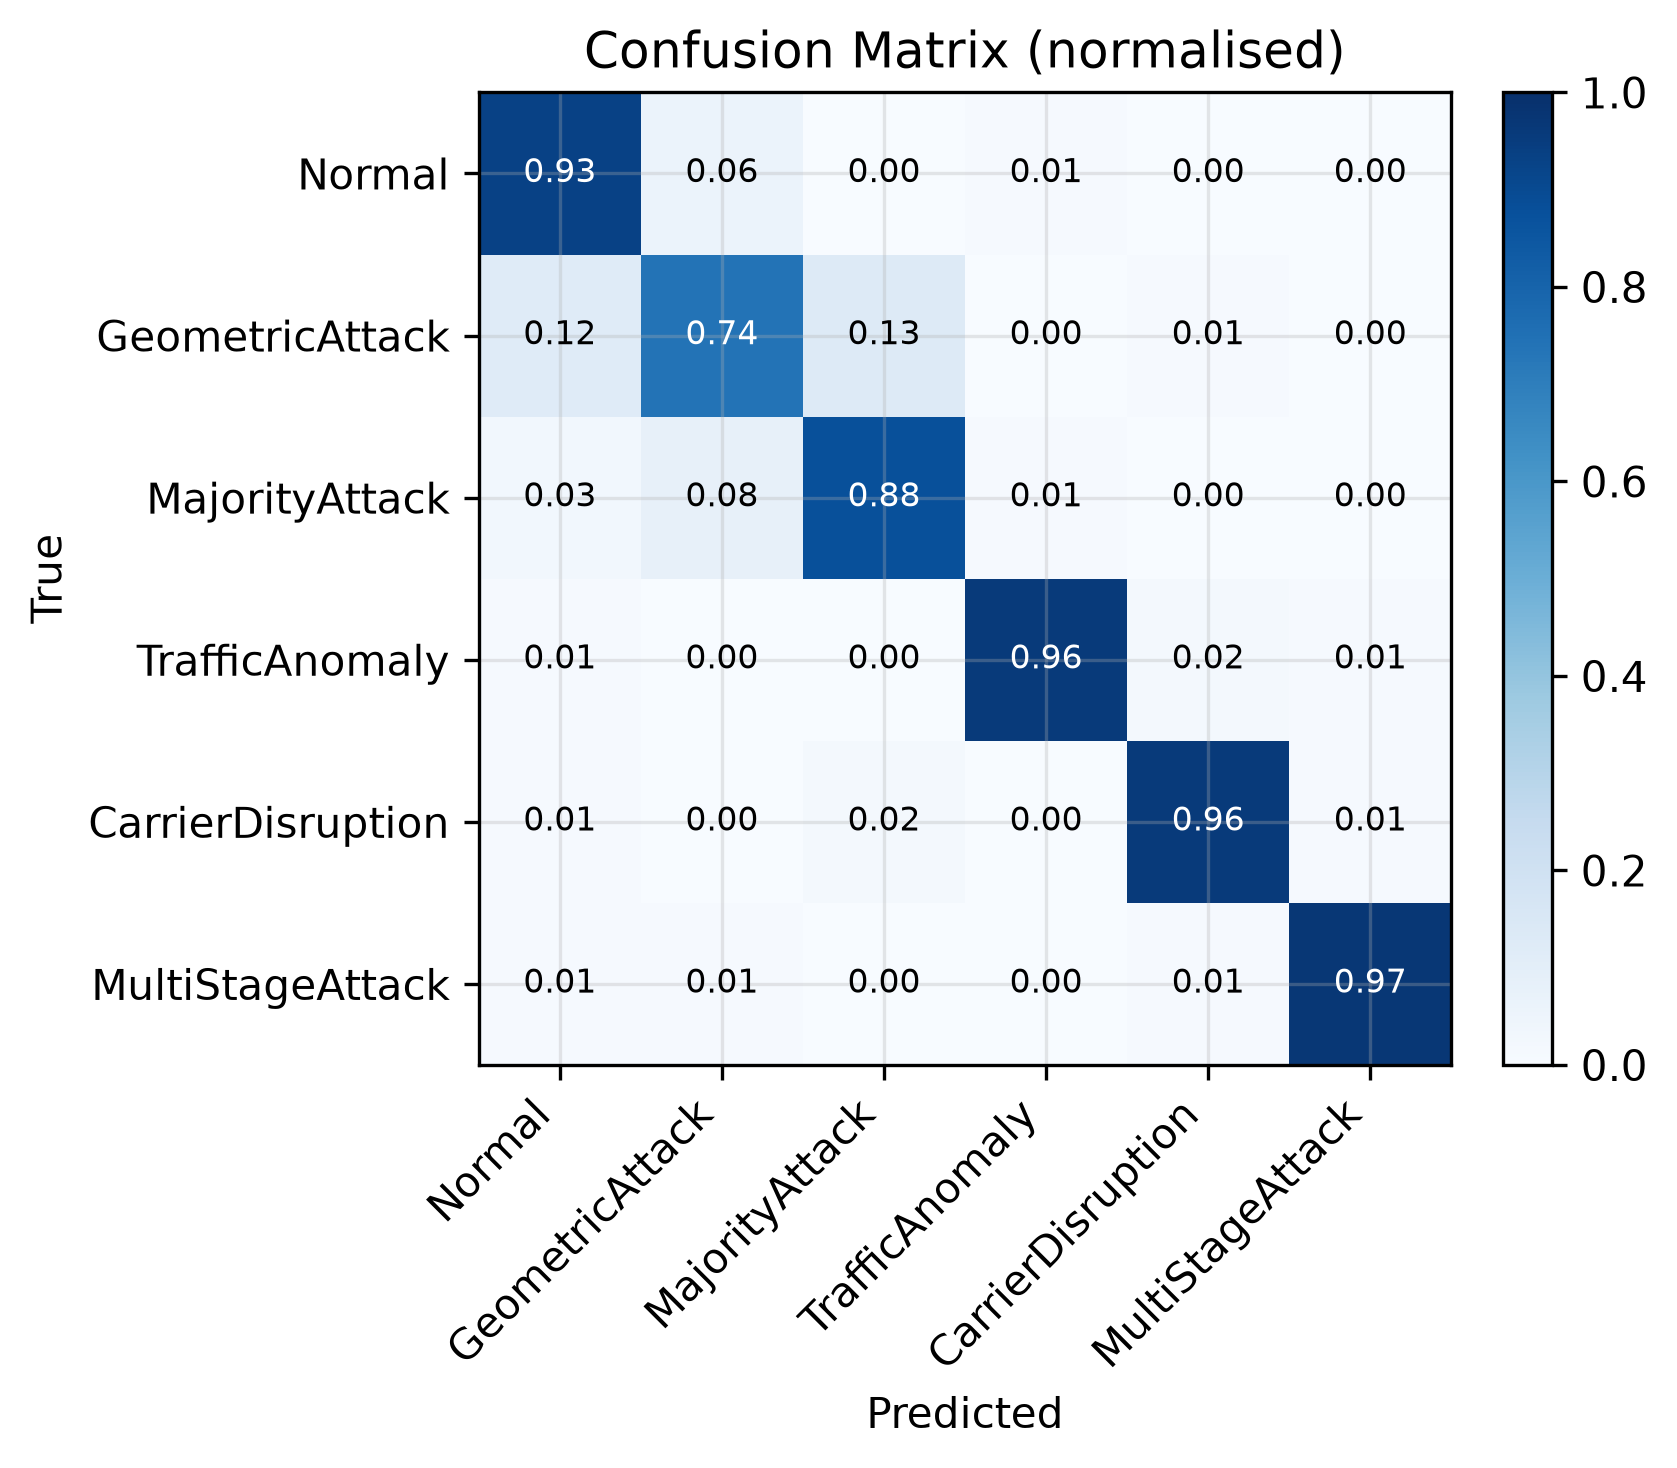
\includegraphics[width=0.49\columnwidth]{confusion_matrix.png}\hfill
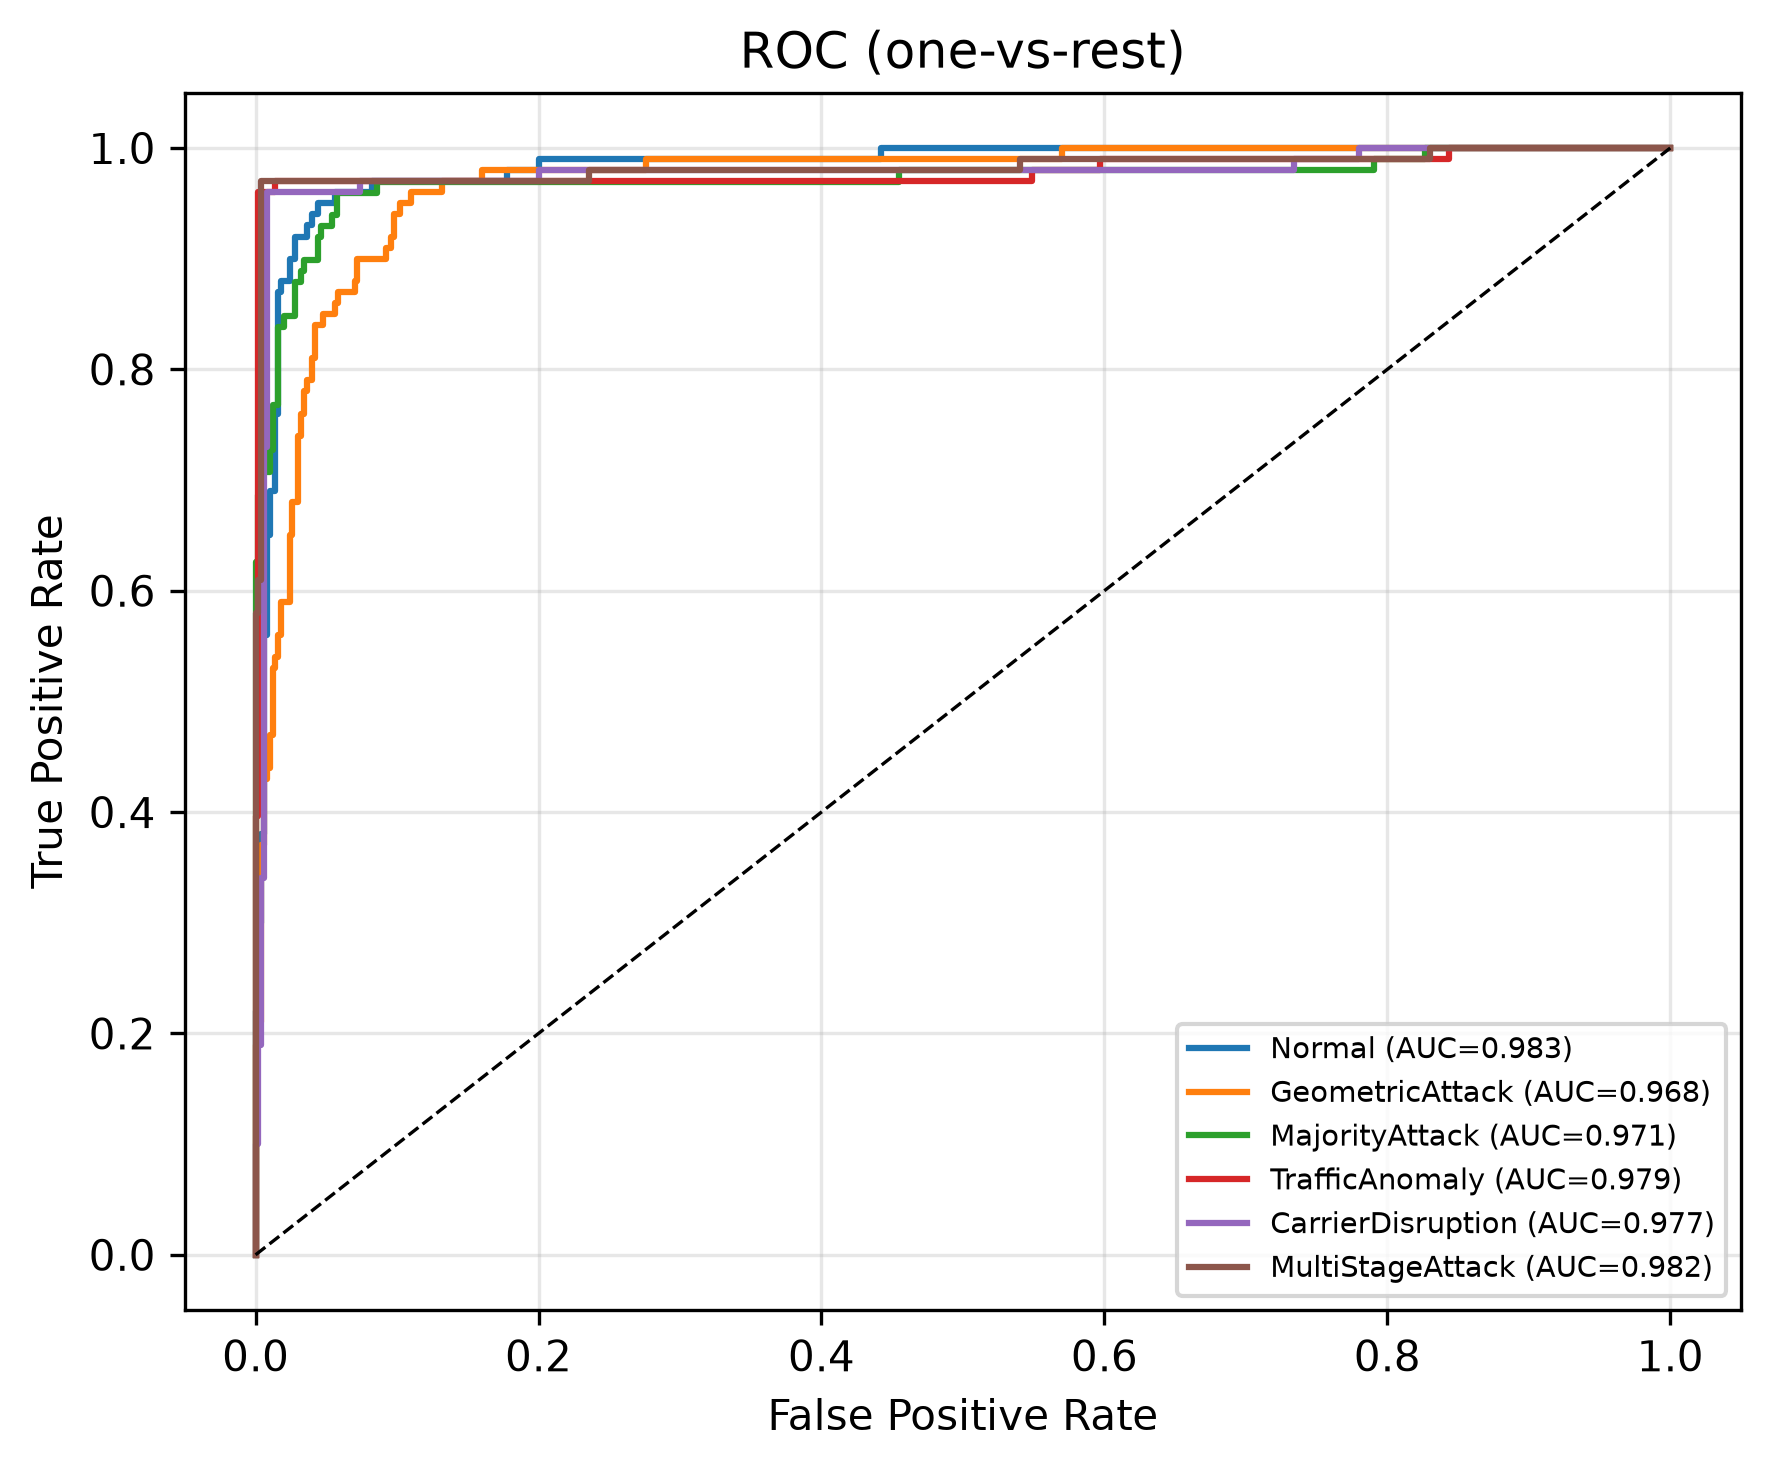
\includegraphics[width=0.49\columnwidth]{roc_curves.png}
\caption{Hybrid detector on the held-out split: normalized confusion matrix (left)
and per-class one-vs-rest ROC curves (right). Macro-averaged ROC-AUC is 0.977.}
\label{fig:det}
\end{figure}

Fig.~\ref{fig:featimp} (left) shows which features carry the most weight---transport
signals dominate the permutation-importance ranking, but dropping either group
degrades performance meaningfully, which is exactly the fusion claim. The weight
analysis (Fig.~\ref{fig:featimp}, right) shows a modest but real gain from mixing
the two base learners rather than relying on either alone.

\begin{figure}[t]
\centering
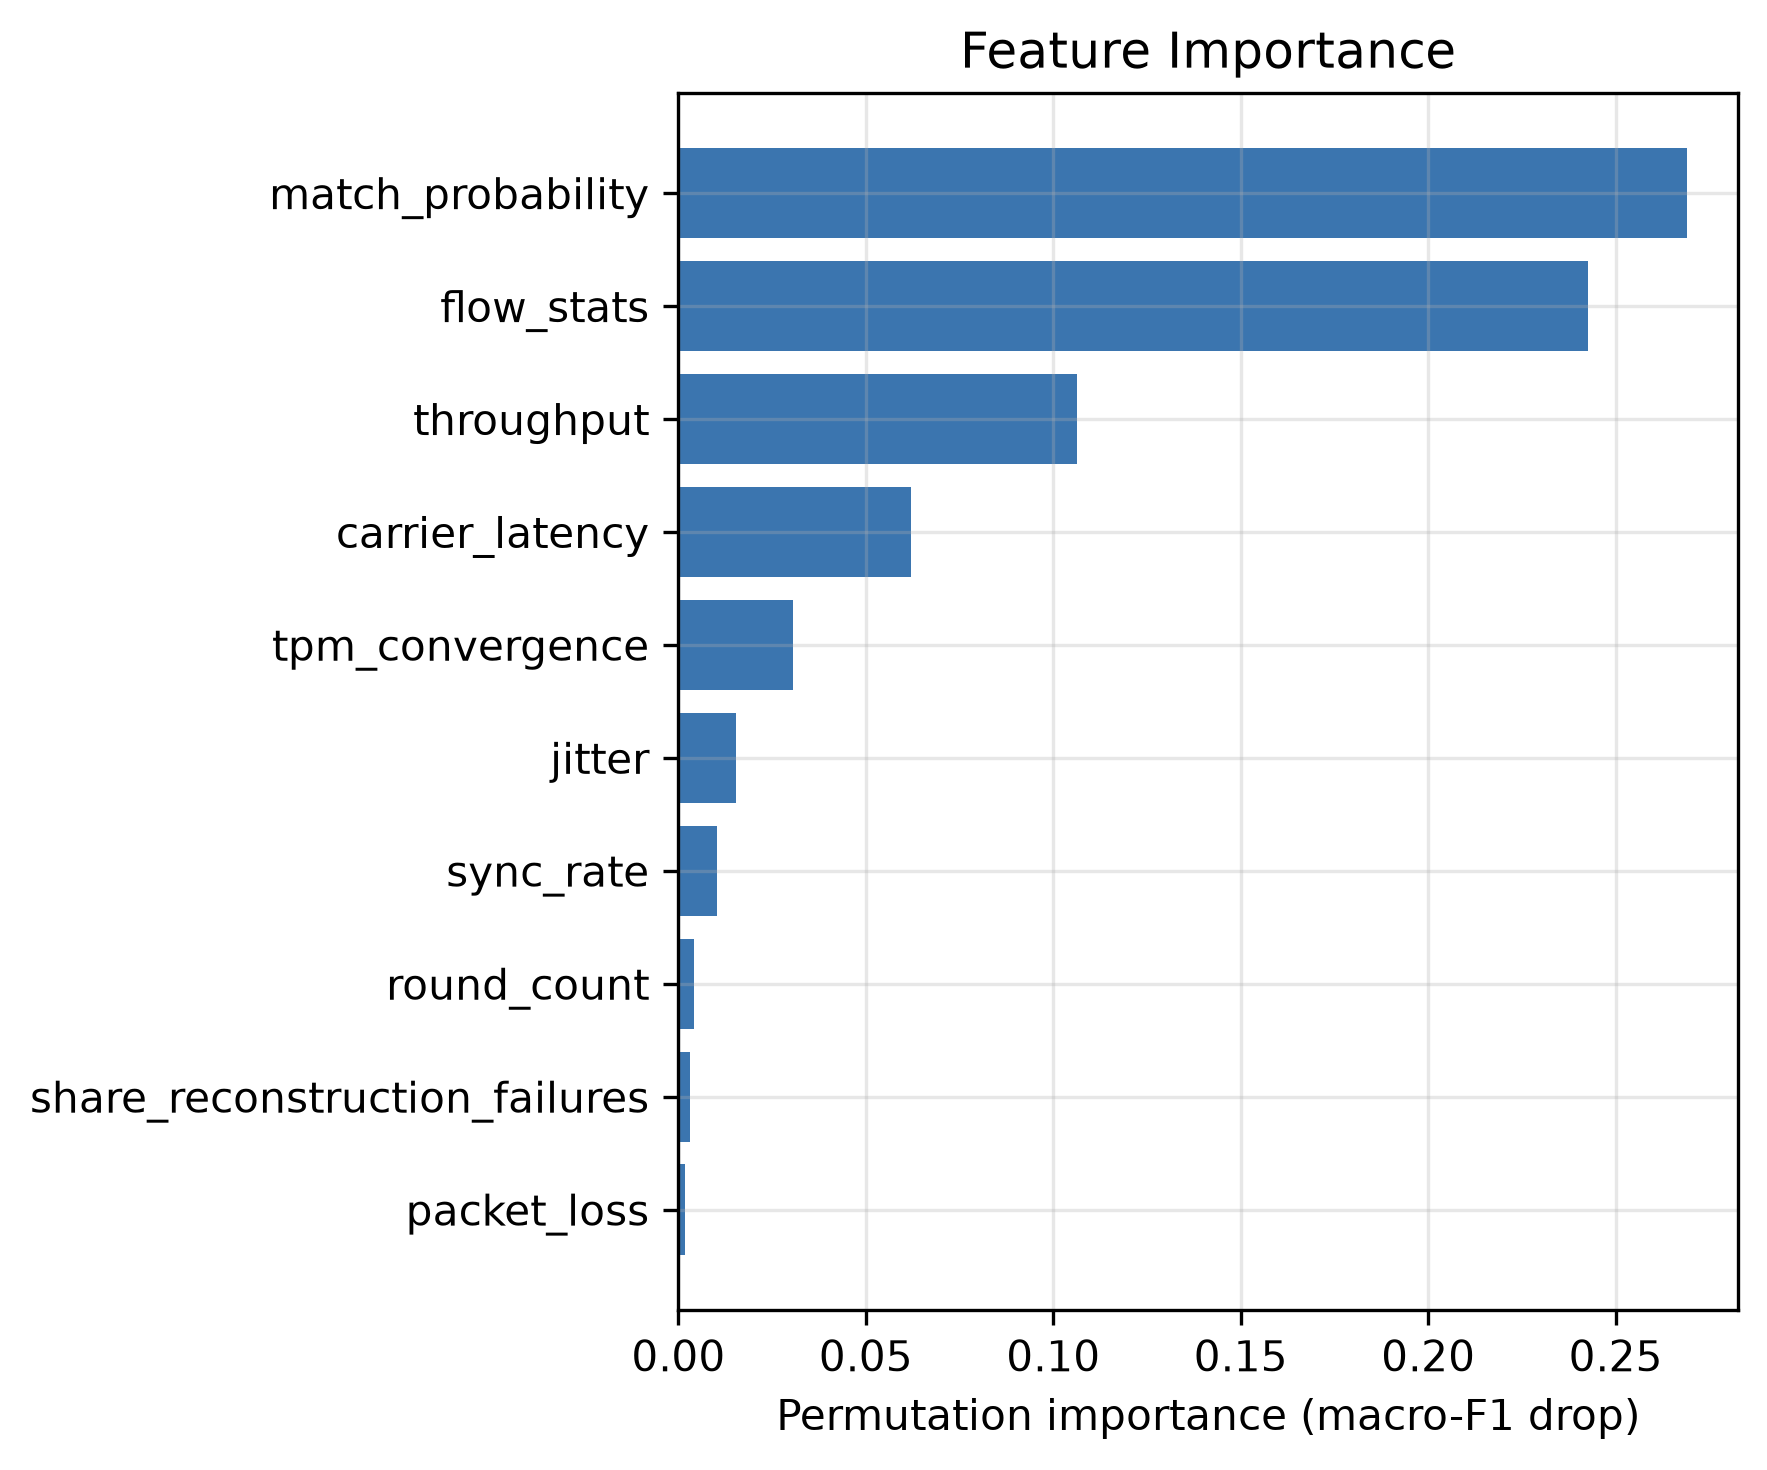
\includegraphics[width=0.49\columnwidth]{feature_importance.png}\hfill
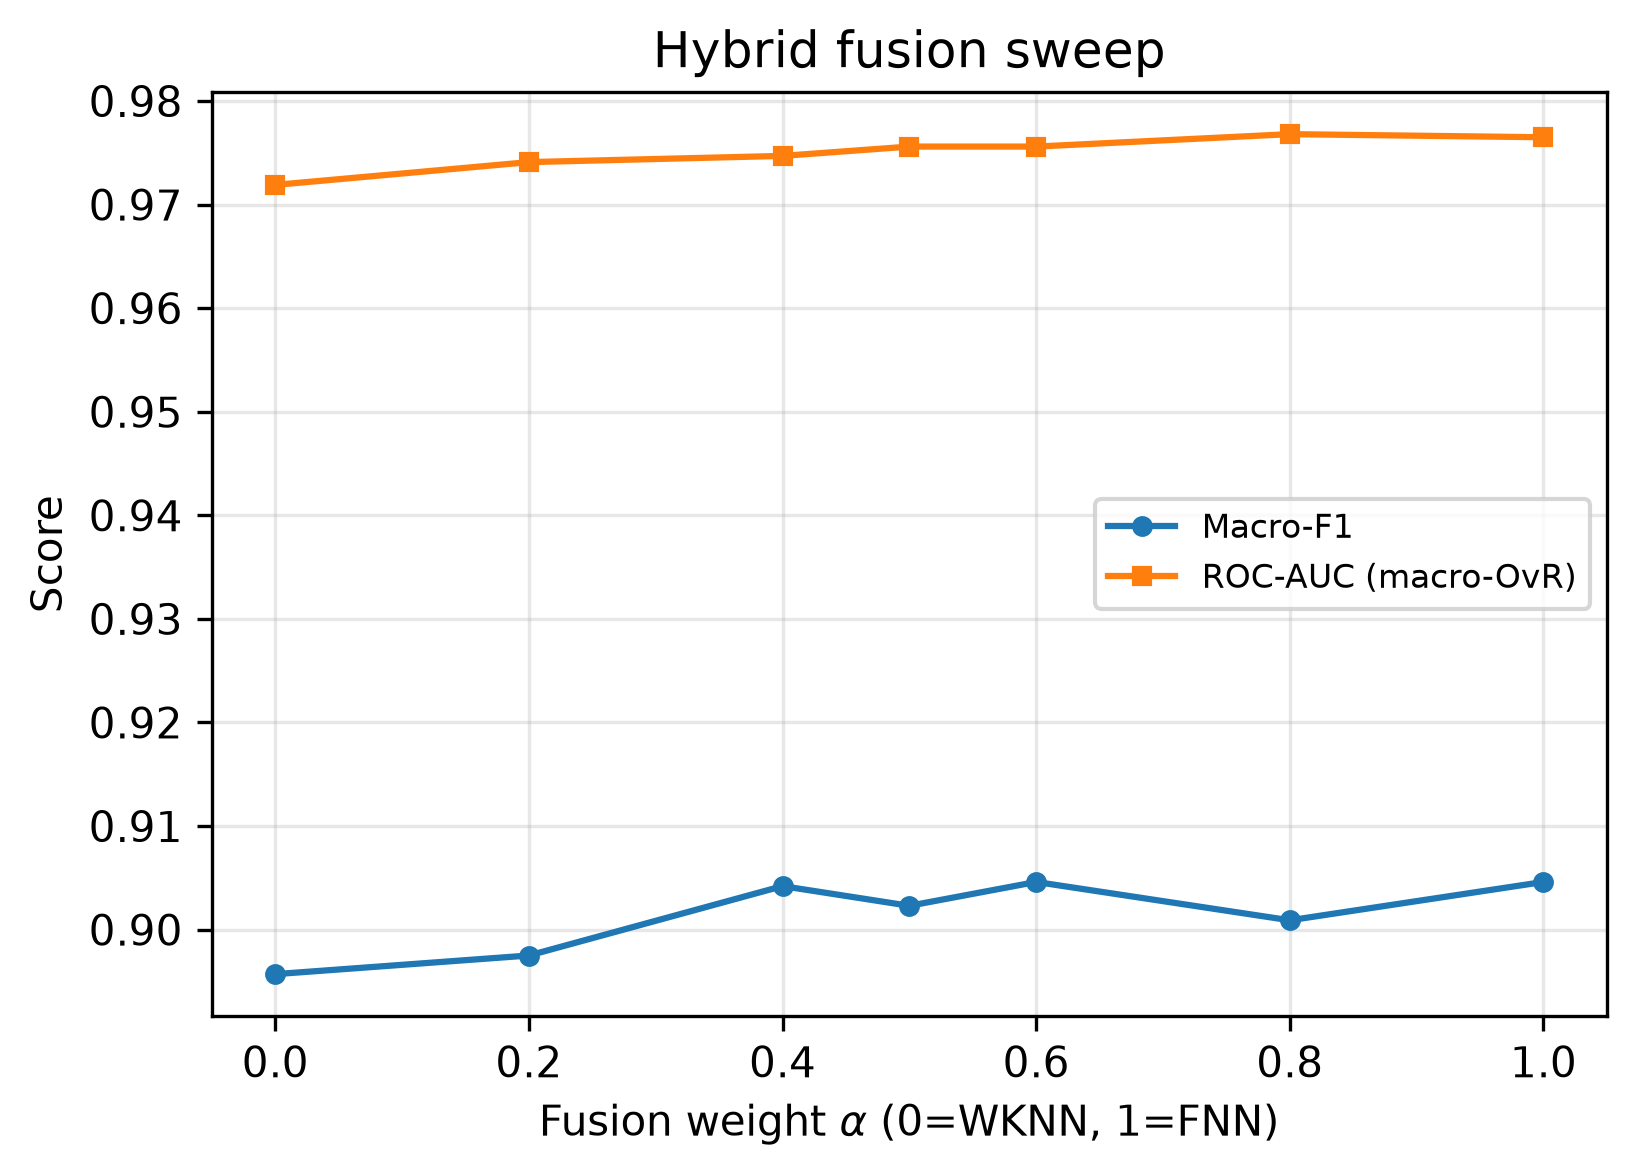
\includegraphics[width=0.49\columnwidth]{sweep_alpha.png}
\caption{Left: permutation feature importance on the held-out split.
Right: macro-F1 and ROC-AUC vs.\ fusion weight $\alpha$ ($0{=}k$NN, $1{=}$FNN);
an intermediate $\alpha$ slightly outperforms either base learner alone.}
\label{fig:featimp}
\end{figure}

The second and arguably more important finding is that the specific classifier
barely matters once the features are right. Table~\ref{tab:baselines} puts our
hybrid next to random forest, RBF-SVM, gradient boosting, and logistic regression,
all on the same features and splits. Every model lands between 0.89 and 0.90
macro-F1, with standard deviations that overlap completely. A McNemar test of the
hybrid against logistic regression---which happened to score highest on the single
test split at 0.911---gives $\chi^2{=}3.06$, $p{=}0.08$, not significant. The
honest conclusion: once you have both telemetry streams, almost any off-the-shelf
classifier will work, and the effort should go into the feature pipeline rather than
the model.

\begin{table}[t]
\centering
\caption{Detector vs standard baselines on the grounded telemetry (mean$\pm$std macro-F1 over 3 seeds, all using both feature modalities). The hybrid matches the field on AUC; a McNemar test against the strongest baseline finds no significant gap ($p{=}0.08$), so the contribution is cross-modal fusion and integration, not classifier superiority.}
\label{tab:baselines}
\begin{tabular}{lcc}
\toprule
Model & Macro-F1 & ROC-AUC \\
\midrule
Random Forest & 0.901$\pm$0.004 & 0.974 \\
SVM (RBF) & 0.903$\pm$0.010 & 0.973 \\
Grad. Boosting & 0.888$\pm$0.010 & 0.974 \\
Logistic Reg. & 0.898$\pm$0.013 & 0.976 \\
WKNN & 0.888$\pm$0.008 & 0.973 \\
FNN & 0.898$\pm$0.010 & 0.976 \\
\textbf{Hybrid (ours)} & 0.896$\pm$0.010 & 0.976 \\
\bottomrule
\end{tabular}
\par\smallskip
{\footnotesize McNemar (hybrid vs logistic): $\chi^2{=}3.0625$, $p{=}0.0801$.}
\end{table}


% ============================================================
\section{Limitations}
% ============================================================

Several things this paper does not claim. Post-quantum confidentiality comes from
ML-KEM; the TPM step is broken by known attacks~\cite{klimov2002analysis,
shacham2004cooperating} and is treated strictly as auxiliary entropy. Passive
eavesdroppers are invisible to the detector by construction---active, host-observable
probing is what we model, not a passive listener. Raising $T$ in the $(T,N)$ scheme
always costs availability (Eq.~\ref{eq:avail}), and no scheme-level trick escapes
that. The main detector results come from grounded synthetic telemetry; 5G-NIDD
evaluation of the fusion path requires augmented cryptographic features and is
therefore semi-synthetic. ML-KEM timings here reflect Python dispatch overhead, not
hardware speed; real on-device numbers need optimized assembly~\cite{kannwischer2019pqm4}.
Finally, genuine path independence for bifurcation requires physically separate
carriers---two modems or operators---not two component carriers behind one shared
radio front-end.

% ============================================================
\section{Conclusion}
% ============================================================

The useful move is to put each piece where it genuinely earns its place and not
oversell what it cannot do. ML-KEM carries the post-quantum guarantee because it has
a proof; TPM contributes auxiliary entropy because it has a wire footprint that ML-KEM
cannot match in the most constrained settings; the $(T,N)$ scheme turns the
confidentiality--availability trade-off from a fixed property into an operator
decision; and a cross-modal detector makes active attacks observable, with fusion
doing the heavy lifting rather than any particular model. What the experiments show
most clearly is that having two kinds of telemetry in the room at the same time is
what enables the detection, not any sophisticated architecture on top of it. The full
artifact---data generator, experiments, deployment path---is provided so these claims
can be checked, not just read.

% \clearpage
\bibliographystyle{IEEEtran}
\bibliography{references}

\end{document}
